\subsection{Definitions Related To Dfg-Method}
In this part, we provides concepts related to the dfg-method which is based on directly-follows graph. A directly-follows graph as used in \cite{leemans2013discovering}, represents the directly-follows relation of activities in event log. For instance, if there are traces of $\langle ...,A,B,... \rangle$ in event log, one edge (A,B) is added into directly-follows graph. By cutting directly-follows graph under different conditions, Inductive Miner\cite{leemans2013discovering,leemans2014discovering} discovers a process model. Unlike this process, we adapt Inductive Miner to repair model by using existing model, and event log with labels.

\begin{definition}[Cardinality in directly-follows graph]
	Given a directly-follows graph G(L) derived from an event log L, the cardinality of each directly-follows relation in G(L) is defined as:  
	\begin{itemize}
		\item $Cardinality(E(A,B))$ is the frequency of traces with $\langle ...,A,B,... \rangle$. 
		\item Start node A cardinality $Cardinality(Start(A))$ is the frequency of traces with begin node A.
		\item End node B cardinality $Cardinality(End(A))$ is the frequency of traces with end node B.
	\end{itemize}	
\end{definition}
From the positive and negative event log, we can get directly-follows graphs, respectively $G(L_{pos})$ and $G(L_{neg})$. Each edge of  $G(L_{pos})$ and $G(L_{neg})$ has a cardinality to represent the strength of this directly-follows relation. 
However, when the existing model is transformed into  directly-follows graph $G(L_{ext})$, there is no point to assign cardinality on each edge. So we just set 1 to cardinality of each edge. 

%To incorporate all information from  $G(L_pos)$, $G(L_neg)$ and $G(L_ext)$, a data structure is defined directly-follows matrix. 
To incorporate all information from  $G(L_{pos})$, $G(L_{neg})$ and $G(L_{ext})$, we define  weight for each directly-follows relation in graph. 
\begin{definition}[Weight of directly-follows relation]
	Given a directly-follows graph G(L), the weight of each directly-follows relation is defined as \[ Weight(E(A,B)) = \frac{Cardinality(E(A,B))}{Cardinality(E(A,*))}  \] 
	for start activities A, we have 
	\[ Weight(Start(A)) = \frac{Cardinality(Start(A))}{Cardinality(Start(*))} \]
	Similarly for end activities B, we have
	\[ Weight(End(B)) = \frac{Cardinality(End(B))}{Cardinality(End(*))} \]
	E(A,*) means all edges with source A, E(*,B) means all edges with target B, Start(*) represents all start nodes, and End(*) represents all end nodes.
\end{definition}
After defining the weights of each directly-follows relation, for each directly-follows relation, there are three weights from $G_{pos}$, $G_{neg}$ and $G_{ext}$. The following strategy assigns new weight to directly-follows relation to new generated directly-follows graph $G_{new}$.
\begin{definition}[Assign new weights to graph $G_{new}$]
	there are three weights from $G_{pos}$, $G_{neg}$ and $G_{ext}$, the new weight is 
	\begin{itemize}
		\item For one directly-follows relation, \[ Weight(E_{G_{new}}(A,B)) = Weight(E_{G_{pos}}(A,B)) + Weight(E_{G_{ext}}(A,B)) - Weight(E_{G_{neg}}(A,B))\]
		\item For start activities A, we have 
		\[ Weight(Start_{G_{new}}(A)) = Weight(Start_{G_{pos}}(A)) + Weight(Start_{G_{ext}}(A)) - Weight(Start_{G_{neg}}(A)) \]
		\item For end activities B, we have
		\[ Weight(End_{G_{new}}(A)) = Weight(End_{G_{pos}}(A)) + Weight(End_{G_{ext}}(A)) - Weight(End_{G_{neg}}(A)) \]
	\end{itemize}
\end{definition}
After assigning all the weight to directly-follows relation in $G_{new}$, we filter out all directly-follows relation in $G_{new}$ with weight less than 0. 
Then, we transform the $G_{new}$ into process tree bu using Inductive Miner for the next stage.

\subsection{Definitions Related To Add Long-term Dependency}
\textit{Example 1} Consider event log L with labels \[L =[\langle A,C,E \rangle^{50,pos}, \langle B,C,D \rangle^{50,pos}, \langle A,C,D \rangle^{50,neg}]. \] $\langle A,C,E \rangle^{50,pos}$ means there are 10 traces $\langle A,C,E \rangle$ labeled as positive in event log. Similarly, $\langle A,C,D \rangle^{50,neg}$ represents there are $\langle A,C,D \rangle$ traces at number 50 in event log which have negative labels. 

After applying the dfg-algorithm, a model as shown in Figure \ref{fig:pn_without_lt_exm01} is discovered. In event log L, B and D has long-term dependency, and A is expected to support only the execution of E, since $<A,C,D>$ is negative and $<A,C,E>$ is positive. However, the model doesn't express those constraints.
\begin{figure}[h!]
	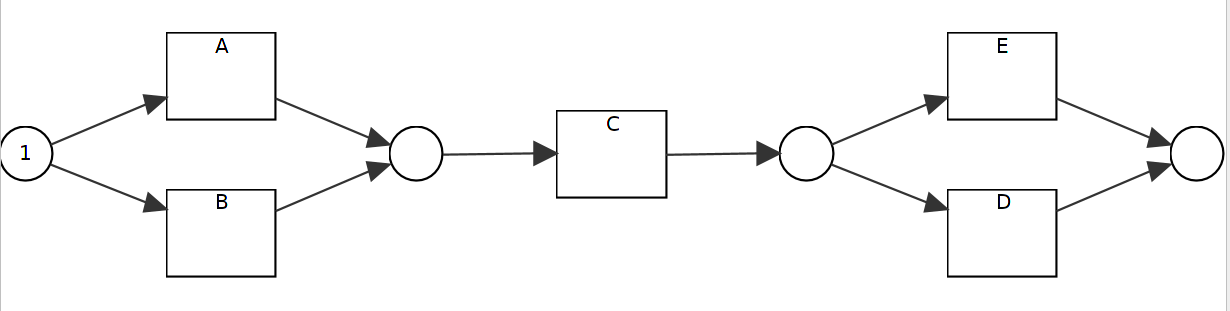
\includegraphics[width=\textwidth]{figures/preliminaries/PN06_Seq_2_xor_notnested.png}
	\caption{Process model generated from dfg-algorithm}
	\label{fig:pn_without_lt_exm01}
\end{figure}
Obviously, long-term dependency relates the choices structure in process model, such as exclusive choice, loop and or structure. Due to the complexity of or and loop structure, only the long-term dependency in exclusive choice is considered. 

The inputs for this algorithm are,
\begin{itemize}
	\item Repaired model in process tree
	\item Event log with positive and negative labels
\end{itemize}
The output of this algorithm is: 
\begin{itemize}
	\item Repaired model in petri net with long-term dependency
\end{itemize}
%%if now, we only consider the repaired process tree model, then we don't have problems to make the weights of dfg and long-term dependency unified. But we have it from the existing model, because of existing factor. 
%% Now we have the firstly-repaired model, if we want to create long-term dependency, we also have the 3 weights:: 
%% Ext_Wlt(Si, Tj), but when our negative factor affects, we need to unify them!!To prove it!!! 

Process tree, as one input for the algorithm, is one common model to interpret business process in process mining. It's a block-structured tree. To specify the process tree with respect to long-term dependency, the following definitions are in need. Firstly, the definitions related to tree are reviewed.
\begin{definition}[Tree]
	Let $ \mathscr{E} $ be a finite set of entities, a tree is a collection of entities called nodes, which are connected by edges. A tree T is,
	
	\begin{itemize}
		\item t, with  $t\in \mathscr{E}$, t has no outgoing edges
		\item $t(T_1,T_2,...,T_n)$, with $t\in \mathscr{E}, i,n\in \mathbb{N}, i \leq n ,T_i$ is a tree.
	\end{itemize}
\end{definition}
$T_i$ is a child or subtree of $t(T_1,T_2,...,T_n)$, $t(T_1,T_2,...,T_n)$ is one parent of $T_i$, which can be expressed in $P(t(T_1,T_2,...,T_n),T_i)$. The root of tree is the node without any parent; A tree has only one root. A leaf node is the node which has no children nodes.\\
For a node in a tree, its ancestor and descendant are defined as:
\begin{definition}[Ancestor Relation Anc(A,t)]
	An ancestor of a node t in a tree is a node A, written as $ Anc(A,t) \Rightarrow True$, if those conditions hold,  
	\begin{itemize}
		\item A is a parent of t, written as $ P(A,t) \Rightarrow True$, or
		\item $\exists t_1,t_2..t_n,n\in \mathscr{E}, i < n, P(A,t_1)\land P(t_i,t_{i+1}) \land P(t_n,t) \Rightarrow True $
	\end{itemize}
\end{definition}
The ancestor of root is empty, while leaf nodes has no descendants. Based on this, we define the ancestors set of a node s. 
\begin{definition}[Ancestors of a node a]
	The ancestors set of a node s, Ancestors(s), is defined as: \[ Ancestors(A)=\{t|Anc(t,s) \Rightarrow True \} \]
\end{definition}
Accordingly, descendant relation is given for node t and node s, Des(s,t). If node s is the ancestor of t, then t is a descent of s. $Anc(s,t) \Rightarrow Dec(t,s)$; The set of descendants of node t is Descendants(t).
\begin{definition}[Least Common Ancestor]
	A least common ancestor for node $s$ and node $t$ in a tree is a node n, where 
	\[Anc(n,s) \land Anc(n,t) \land \exists! m Anc(n,m) \land Anc(m,s) \land Anc(m,t) \]
\end{definition}

In process tree, all the leaves are activities in business process, and the middle nodes are operators which represents the relations of all its children nodes\cite{vanderAalst:2016:PMD:2948762,leemans2013discovering}. This paper uses four operators in context of long-term dependency. The four relations.  $\{\rightarrow, \times, \land, \circlearrowright\}$ are considered. 

Next, we only focus on exclusive xor structure on long-term dependency. As known, long-term dependency is associated with choices. In xor block, it means the choices of each xor branch in xor block. For sake of convenience, we define the xor branch.

$Q= \times(Q_1 , Q_2 ,.. Q_n)$, $Q_i$ is one xor branch with respect to Q, rewritten as $XORB_{Q_i}$ to represent one xor branch $Q_i$ in xor block, and record it $XORB_{Q_i} \in XOR_{Q}$. For each branch, there exists the begin and end nodes to represent the beginning and end execution of this branch, which is written respectively as Begin($XORB_{Q_i}$) and End($XORB_{Q_i}$).

%% but the structure of xor branch, do we need to think of right now?? we need to think of it 
For convenience of analysis, two properties of xor block, purity and nestedness are demonstrated to express the different structures of xor block according to its branches.
\begin{definition}[XOR Purity and XOR Nestedness] The xor block purity and nestedness are defined as following: \\
	\begin{itemize}
		\item A xor block $XOR_Q$ is pure if and only $\forall XORB_X \in XOR_Q, XORB_X $ has no xor block descent, which is named as pure xor branch. Else,
		\item A xor block $XOR_Q$ is nested if $ \exists XOR_X, Anc(XOR_Q, XOR_X) \rightarrow True  $. Similarly, this xor branch with xor block is nested.
	\end{itemize}
\end{definition}
%% change the graph for whole explaination!!
In the Figure\ref {fig:xor_nested_branch_variants}, xor block Xor(c1,c2) are pure and not nested, since all the xor branches are leaf node, but xor block Xor(a,Seq(b,Xor(c1,c2))) is impure and nested with Xor(c1,c2). 
\begin{figure}[h!]
	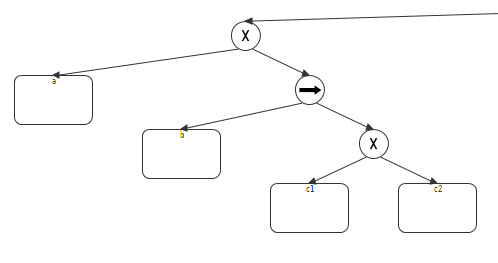
\includegraphics[width=\textwidth]{figures/preliminaries/PT02_xor_nested_and_pure.png}
	\caption{XOR branch variants}
	\label{fig:xor_nested_branch_variants}
\end{figure}

%% xor branch, the dependency between them, then how about the dependency on that part, does it exist in the xor block, so we can define it ??
%% the full completeness is also dependency, but sth different, 
%% for arbitrary two xor branches, if they are long-term dependency?? Can I decide, or not ?? I can decide it!! But in the specific way, if they are in a pair, they are ok, else, not !!! 
%% but it goes far, so only write down what I have achieved, but in their thinking way, why in my way?? 
%% given two branch, and they have order, just complexity of implementation, then we only consider the directly ones!!  

Long-term dependency researches on the dependency of choices in xor block, with observation, actually on the pure xor branch, because nested xor branch has multiple choices, which affect the execution of later process. For two arbitrary pure xor branches, to have long-term dependency, they firstly need to satisfy the conditions: (1) they have an order;(2) they have significant correlation.
The order of xor branch follows the same rule of node in process tree which is explained in the following.
\begin{definition}[Order of nodes in process tree]
	Node $X$ is before node $Y$, written in $X \prec Y$, if $X$ is always executed before $Y$.  In the aspect of process tree structure, $X \prec Y$, if the least common ancestor of $X$ and $Y$ is a sequential node, and $X$ positions before $Y$.
\end{definition} 
%% how to define the correlation fo xor branches, if they always happen together
The correlation of xor branches is significant if they always happen together. To define it, several concepts are listed at first. 
\begin{definition}[Xor branch frequency]
	Xor branch $XORB_X$ frequency in event log l is $F_{l}(XORB_X)$, the count of traces with the execution of $XORB_X$. \\
	For multiple xor branches, the frequency in event log l is defined as the count of traces with all the execution of xor branches $XORB_{Xi}$ , written as \[F_{l}(XORB_{X1}, XORB_{X2},...,XORB_{Xn})\].
\end{definition}
%% correlation means the two always happen together, if one not shown, the other also not?? So the connection support.. how to define them?? 
%% connection support, we can say only on number, when it is over one value, 
After calculation of the frequency of the coexistence of multiple xor branches in positive and negative event log, we get the supported connection of those xor branches, and define the correlation. 
\begin{definition}[Correlation of xor branches]
	\label{def: supported-connection}
	For two pure xor branches, $XORB_X \prec XORB_Y$, the supported connection is given as \[SC(XORB_X,XORB_Y)= F_{pos}(XORB_X, XORB_Y) -F_{neg}(XORB_X, XORB_Y)\]. If $SC(XORB_X,XORB_Y) > lt-threshold$, then we say $XORB_X$ and $XORB_Y$ have significant correlation.
\end{definition}

I did some introduction, it is proven that in some cases, we can't deal with it. When the $XORB\_S \neq LT\_S || XORB\_T \neq LT\_T$.

Another way to avoid this problem is to add duplicated events, but the problem stays the same, so if we want to keep the model fit, we add new event for the discovered long-term dependency, the original, we keep it in the model?? But it is not precise!!! It allows too many choices there, but the model is sound, because we add events on model, we produce and consume tokens from duplicated events, and consumes it later.. Still, it is not so right. But if we choose the events before, we decides the events later, it's true... helps a little... 

How to prove it ?? By induction. 
We use  process  trees as one internal result in  our  approach in two factors: (1) they are sound by construction, and can be transferred into sound Petri net models; (2) they are block-structured. which benefits the detection of exclusive relations in model.

\begin{itemize}
	\item the original model is sound
	\item after adding one long-term dependency by duplicating the event, we make sure
	 \\ duplicated events are added into the xor branches, if it's chosen, then it consumes one token, at this xor branches, then it produces two tokens, one of which is put back again into the 
	 To prove the added places and duplicated events between two xor branches will not violate the soundness of model. 
	 \item 
	 \begin{itemize}
	 	\item adding duplicated events of one long-term dependency does not violate the soundness of model. 
	 	
	 	\item To connect the source and target  of long-term dependency which are the duplicated events will not violate the soundness.
	 	\\ One extra place is added to connect the source and target. After executing the source, one token is generated in this place; Due to long-term dependency, only this target is triggered by this token and it consumes this token. No extra token is introduced into this model, so the model keeps sound. 
	 	
	 \end{itemize}
	 
	 \item While keeping the original event in the model,  the model is with less precision.  
	 \\ 
	 So I want to solve this problem, and make it preciser by considering the original events into model... 
	 One drawback exists there, still... If we use the old and then the 
\end{itemize}

It's about 12 pages. But one problem, some basic information, we forget to give .. Maybe, we can put the related work later!!!

